
\documentclass[12pt]{article}
\usepackage{geometry} % see geometry.pdf on how to lay out the page. There's lots.
\usepackage{subfig}
\usepackage{parskip}
\usepackage{graphicx}


\geometry{letterpaper} % or letter or a5paper or ... etc
% \geometry{landscape} % rotated page geometry

% See the ``Article customise'' template for come common customisations

\title{Expertise in Recommender Systems}
\author{Chaofei Fan, Jiasi Zeng}
%\date{} % delete this line to display the current date

%%% BEGIN DOCUMENT
\begin{document}

\maketitle

%%%%%%%%%%%%%%%%%%%%%%%%%%%%%%%%%%%%%%%%%%%%%%%%
% Section 1
%%%%%%%%%%%%%%%%%%%%%%%%%%%%%%%%%%%%%%%%%%%%%%%%
\section{Introduction}
Recommender System is becoming a crucial part of our online experience these days. It is widely used in various websites to recommend all kinds of products to customers: movies\footnote[1]{www.flixster.com}, books\footnote[2]{www.amazon.com}, music\footnote[3]{www.pandora.com}, etc. The quality of a recommender system is not only related to user experience, but also revenues of online business.  

Different recommendation methods have been proposed in both industry and academia. The performance of recommender systems is usually measured with two metrics: accuracy and coverage. Higher accuracy means the estimated rating of one item for target user is more likely to match the user's own rating of that item; higher coverage means the system is able to predict more items' ratings for more users. 

One of the most popular recommendation method is Collaborative Filtering (CF) \cite{Sarwar:2001p125}. CF compares rating profiles of all items and identifies \emph{similar items} using similarity measure like \emph{Pearson Correlation}. For example, in item-based CF, when asked to predict the rating of a target item for a target user, CF first finds items which are similar to the target item, then it returns the target user's average ratings of these similar items (weighted by their similarities to the target item). Though CF has been adopted by many recommender systems, it performs poorly for cold-start users (i.e. new users of a website who has rated few items). Since cold-start users have rated only a few items, it is often difficult for CF to find similar items rated by the target user. Therefore, coverage of CF is usually very low for cold-start users. 

To overcome the weakness of CF on cold-start users, Mohsen Jamali and Martin Ester proposed Trustwalker \cite{Jamali:2009p67}. Trustwalker combines trust-based method and item-based CF by performing a random walk on the target user's neighbours (both direct and indirect). TrustWalker substantially improves the coverage of existing trust-based approaches while maintaining the same or even slightly better precision.

To explore potential improvement in these recommender systems mentioned above, we propose a new recommendation method, which utilizes users' expertise in different product categories. The rationale behind this method is that experts' reviews tend to be more insightful and cover more items. Besides, according to consumer psychology, consumers tend to trust more on experts when they are purchasing more expensive products, such as cars, electronics, etc \cite{consumer}. Previous research on experts identification in a social network is based on either external data source \cite{Amatriain:2009p101} or implicit user behaviour \cite{Cho:2007p102}. The Epinions.com dataset we crawled contains ratings for reviews, which can be used to determine the quality of reviews. We propose an expert identification algorithm using the quality and number of reviews to find out experts in a certain category. With the identified experts, we make recommendation based on their opinions.

The rest of the report is organized as follows: section 2 introduces the methodology of our expert recommender; section 3 reports the dataset we crawled from Epinions.com and our experiment results on that dataset; section 4 concludes the project. 

%%%%%%%%%%%%%%%%%%%%%%%%%%%%%%%%%%%%%%%%%%%%%%%%
% Section 2
%%%%%%%%%%%%%%%%%%%%%%%%%%%%%%%%%%%%%%%%%%%%%%%%
\section{Methodology}
This section introduces the key steps in the project. 

\subsection{Identifying Experts} % (fold)
\label{sub:identifying_experts}

Given a category $C$ and a set of users $U = \{{u_{1}, ..., u_{n}}\}$ who have written at least one review in category $C$, we primarily consider two factors in calculating a user's expertise: (1) the average quality of the user's reviews, and (2) the total number of user's reviews. We use the following formulas to calculate a user's expertise in a category $C$:
\begin{equation}
E(u) = \frac{\sum_{i=1}^n R_{u, i}} {n} \times f(n)
\end{equation}
\begin{equation}
f(n) = \frac{1}{1 + e^{\frac{-10n} {MAX\_REVIEWS(C)}}}
\end{equation}
where $R_{u, i}$ is the rating for user $u$'s review $i$ in category $C$ and $f(n)$ is a sigmoid function to avoid favoring the number of reviews too much. It is based on the assumption that a user written 100 reviews has more expertise than a user written 10 while a user written 1000 reviews is almost as good as a user written 900 reviews. $MAX\_REVIEWS(C)$ is the maximum number of reviews per user in category $C$. $f(n)$ is tailored for every category, i.e., the user who has written the most reviews in a category have $f(n)=1$.

% subsection identifying_experts (end)

\subsection{Top-$k$ Experts Recommendation} % (fold)
\label{sub:expert_recommendation}

Previous research has demonstrated that recommending items to users based on \emph{expert} opinions can be as good as traditional user-based \emph{Collaborative Filtering} \cite{Amatriain:2009p101}. We propose a similar expert recommendation algorithm: given an item $i$ that belongs to a category $C$, the recommender first picks out the top $k$ percent experts in category $C$; then for each expert, if the expert has rated item $i$, the exact rating is returned; otherwise a weighted average of similar items of $i$ is returned; finally the recommender averages the ratings of all selected experts by their expertise as the predicted rating for item $i$. 

Item similarity is calculated using \emph{Pearson Correlation}:
\begin{equation}
	corr(i,j) = \frac{\sum_{u \in U_{i,j}} (r_{u,i} - \bar{r}_u)(r_{u,j} - \bar{r}_u)} {{\sqrt{\sum_{u \in U_{i,j}} (r_{u,i} - \bar{r}_u)}} \sqrt{\sum_{u \in U_{i,j}} (r_{u,j} - \bar{r}_u)}}
\end{equation}
where $U_{i,j}$ is the set of common users who have rated both items $i$ and $j$, and $\bar{r}_u$ denotes the average of ratings expressed by $u$. Pearson correlation $corr(i,j)$ is in the range $[-1,1]$. Negative correlation means that two items are correlated. Thus we only consider positive correlation.

When predicting the item $i$'s rating for user $u$, the recommender consults the opinions from the set of experts $E = \{e_1, e_2, ...\}$. If expert $e$ has rated the target item $i$, the prediction is calculated directly as:
\begin{equation}
	\hat{r}_{e,i} = \bar{r}_u + (r_{e,i} - \bar{r}_e)
\end{equation}
where $\bar{r}_u$ is the average rating of user $u$ and $\bar{r}_e$ is the average rating of expert $e$. If expert $e$ has not rated the target item $i$, the prediction is calculated using weighted average of similar items rated by the expert:
\begin{equation}
	\hat{r}_{e,i} = \bar{r}_u + \frac{\sum_{j \in I_{sim}} (r_{e,j} - \bar{r}_e) \times corr(i,j)} {\sum_{j \in I_{sim}} corr(i,j)}
\end{equation}
where $I_{sim}$ is the item set similar to item $i$. The recommender aggregates all the experts opinions as the final prediction for user $u$:
\begin{equation}
	\hat{r}_{u,i} = \frac{ \sum_{e \in E} \hat{r}_{e,i} \times exp(e) } { \sum_{e \in E} exp(e) }
\end{equation}
where $exp(e)$ is the expertise of expert $e$.

We also implemented a simple version of top-$k$ experts recommendation. In this version, when predicting a rating of item $i$ for user $u$, the recommender only consults experts who have rated the target item $i$. Experts who have only rated similar items of $i$ are not consulted.
 
% subsection expert_recommendation (end)



%%%%%%%%%%%%%%%%%%%%%%%%%%%%%%%%%%%%%%%%%%%%%%%%
% Section 3
%%%%%%%%%%%%%%%%%%%%%%%%%%%%%%%%%%%%%%%%%%%%%%%%
\section{Experiment}
We tested different recommender systems on a comprehensive dataset from Epinions.com, which is a product reviewing site for consumers. This section reports our findings in the experiments.  
\subsection{Dataset}
Epinions.com is a website where users can rate products and write reviews. Its product catalogue covers a large number of product categories, including Music, Books, Movies, Automobiles, Electronics, etc. For each product, consumers provide ratings on a scale from 1 to 5 (5 being the best), write detailed reviews on products and express the helpfulness of existing reviews. Besides, users can express directed trust among each other: if user A trusts user B, user B does not have to trust user A. In other words, there is a implicit directed trust graph among all users. 

We crawled a comprehensive dataset from Epinions.com, which includes user info, product reviews, review helpfulness, trust links, etc. The size of the crawled dataset is shown in Table \ref{data_size}. Among all the 91,584 users, about 1000 users have written more than 100 reviews. These top 1000 most productive users have contributed to 55.9\% reviews (338,173 out of 605,066).  Table \ref{rating_distro} shows the distribution of ratings among all products. One third of the ratings are 5, and about 60\% of the ratings are 4 or 5. The distribution is very different from another popular dataset -- MovieLens, whose rating distribution is more diverse\footnote[1]{http://www.grouplens.org/node/73}. Table \ref{helpful_distro} shows the helpfulnesses of all reviews. Similarly, about 75\% of all reviews are considered \emph{very helpful}. 

Table \ref{category_distro} shows the number of reviews in the top 5 categories. The top 5 categories account for more than half of all reviews on Epinions.com.

\begin{table}
	\centering
	\subfloat[Dataset Size\label{data_size}] {
		\begin{tabular}[b] {| l | r | }
			\hline
			Data Type & Size \\ \hline \hline
			Users & 91,584 \\ \hline
			Reviews & 605,066 \\ \hline
			Trust Links & 1,152,095 \\
			\hline
		\end{tabular}
	}	
	\subfloat[Rating Distribution\label{rating_distro}] {	
		\begin{tabular}[b] {| c | r |}
		\hline
		Rating & Percentage \\ \hline \hline
		5 & 33\% \\ \hline
		4 & 27\% \\ \hline
		3 & 20\% \\ \hline
		2 & 13\% \\ \hline
		1 & 7\% \\
		\hline
		\end{tabular}
	}
	\subfloat[Review Helpfulness Distribution \label{helpful_distro}] {		
		\begin{tabular}[b] {| l | r | }
		\hline
		Review Helpfulness & Percentage \\ \hline \hline
		Very Helpful & 74.3\% \\ \hline
		Helpful & 15.4\% \\ \hline
		Somewhat Helpful & 6.8\% \\ \hline
		Show & 2.4\% \\ \hline
		Not Yet Rated & 1\% \\
		\hline
		\end{tabular}
	}

	\caption{Dataset Summary}
\end{table}

\begin{table}[h]
	\centering
	\begin{tabular} {| l | c | r | }
		\hline
		Category & Number of Reviews & Percentage \\ \hline \hline
		Movies & 102,461 & 16.9\% \\ \hline
		Books & 72,940 & 12.1\% \\ \hline
		Music & 63,424 & 10.5\% \\ \hline
		Hotels \& Travel & 32,348 & 5.3\% \\ \hline
		Electronics & 31,853 & 5.3\% \\
		\hline
	\end{tabular}
	\caption{Product Categories of Reviews}
	\label{category_distro}
\end{table}

To test the performance of recommender systems, we split the dataset into a training set and a testing set. Testing set is chosen randomly from all ratings and takes about 20\% of all ratings; training set is the rest, which is about 80\%. Then we used the training set to predict the ratings in the testing set. To make the prediction more challenging, we pick out the ratings for controversial items from the testing set and measure the performance separately for these items. We define \emph{controversial items} to be the items whose ratings' Standard Deviations are greater than 1.5 \cite{Massa:2007p437}. These items' ratings are harder to predict, because users' opinions towards these items varies wildly from 1 to 5. The reason why we set a separate testing set for controversial items is that the ratings on Epinions.com are clustered around 4 and 5. Therefore, performing another experiment on controversial items could bring more insight on how the nature of this dataset affects the recommendation methods' performance. 

%%%%%%%%%%%%%%%%%%%%%%%%%%%%%%%%%%%%%%%%%%%%%%%%

\subsection{Evaluation Metrics}

We used two most adopted metrics to measure the performance of recommender systems: Root Mean Square Error (RMSE) and coverage. In addition, we combined \emph{RMSE} and \emph{coverage} into a single metric called F-Measure \cite{Jamali:2009p67}. We define \emph{precision} and \emph{F-Measure} similarly:
\begin{equation}
Precision = 1 - \frac{RMSE}{4}
\end{equation}

\begin{equation}
F-Measure = \frac{2 \times Precision \times Coverage}{Precision + Coverage}
\end{equation}

The next subsection reports the performance of different recommender systems in the Epinions.com dataset. 

%%%%%%%%%%%%%%%%%%%%%%%%%%%%%%%%%%%%%%%%%%%%%%%

\subsection{Experimental Design}
Besides two \emph{Top-k expert} methods, we also implemented item-based CF and Trustwalker to compare the performance. The four methods in our experiments are:

\begin{enumerate}
	\item \emph{itemCF}: This is the traditional CF method, which returns the weighted average ratings of similar items from target user's rating profile. 
	\item \emph{Trustwalker}: This is the random walk model proposed by Mohsen Jamali and Martin Ester \cite{Jamali:2009p67}. We set $max\_depth=3$ and $\sigma=0.001$ in their \emph{Trustwalker} model.
	\item \emph{expert}: This method finds the top-k experts in each category, then calculates weighted average of experts' ratings for target item and also similar items. The estimated rating is adjusted according to target user's rating scale. 
	\item \emph{expert-simple}: This is the simpler version of \emph{expert} method. It finds the top-k experts in each category, and returns the experts' weighted average ratings for the exact target item. The estimated rating is adjusted according to target user's rating scale. 
\end{enumerate}

We also implemented a version of Trustwalker that utilizes the expertise of each user, and return user's rating weighted by their expertise. However, this method performs almost exactly the same as the original Trustwalker. Thus, the results are not shown in this report. 

%%%%%%%%%%%%%%%%%%%%%%%%%%%%%%%%%%%%%%%%%%%%%%%%%

\subsection{Experimental Results}

In this subsection, we present the results of our experiments.

Figure \ref{fig:rmse_all} shows how choosing different expert percentage influences the RMSE of \emph{expert} and \emph{expert-simple}. Table \ref{tbl:compare_all} summarizes the comparison of each methods according to three evaluation metrics.

Figure \ref{fig:sub_rmse_all} and \ref{fig:sub_rmse_cold} shows the RMSE of the four methods over the entire testing set. The horizontal axis represents the percentage of experts we pick from the expert sets. If the percentage is k\%, it means that we take the top k\% of experts with the highest expertise from each category. The category with the largest number of experts is \emph{Movie}, which contains more than 9000 experts, while the category with the smallest number of experts is \emph{Education}, which has roughly 900 experts. So picking top 1\% experts in both category means 90 experts in \emph{Movie} and 9 users in \emph{Education}. Note that both item-based CF and TrustWalker are not affected by the expert percentage, so the RMSE of these two methods are plotted as straight horizontal lines. Note that for \emph{expert} method, we only measured its performance up to 30\% experts due to the limitation of time.

\begin{figure}[htbp]
	\centering
	\subfloat[RMSE for ALL users on ALL items]{\label{fig:sub_rmse_all}
			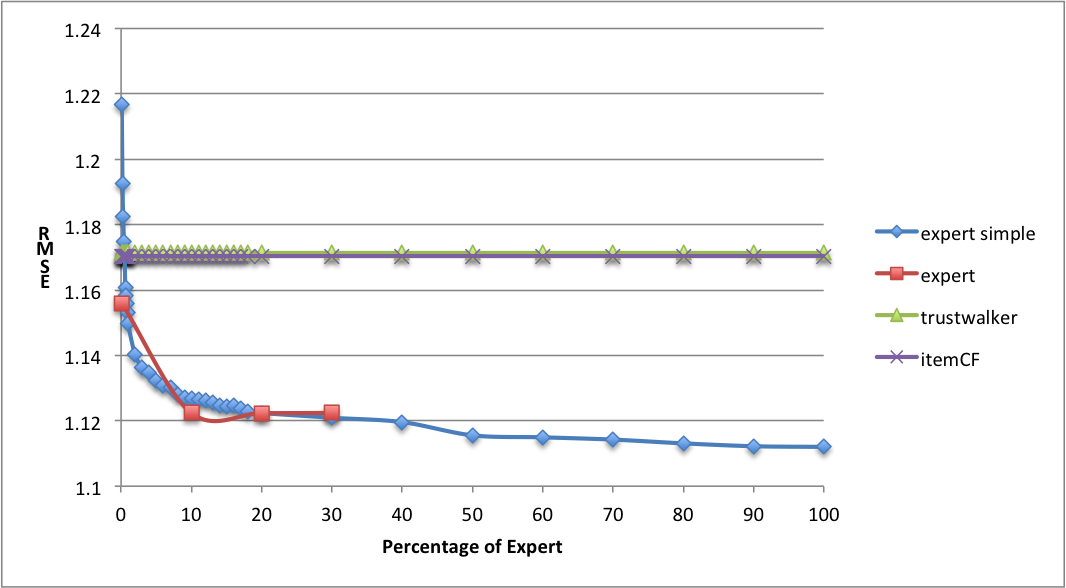
\includegraphics[width=12cm]{graphics/all_user_2.png}			
	}
	\\
	\subfloat[RMSE for COLD-START users on ALL items]{\label{fig:sub_rmse_cold}
			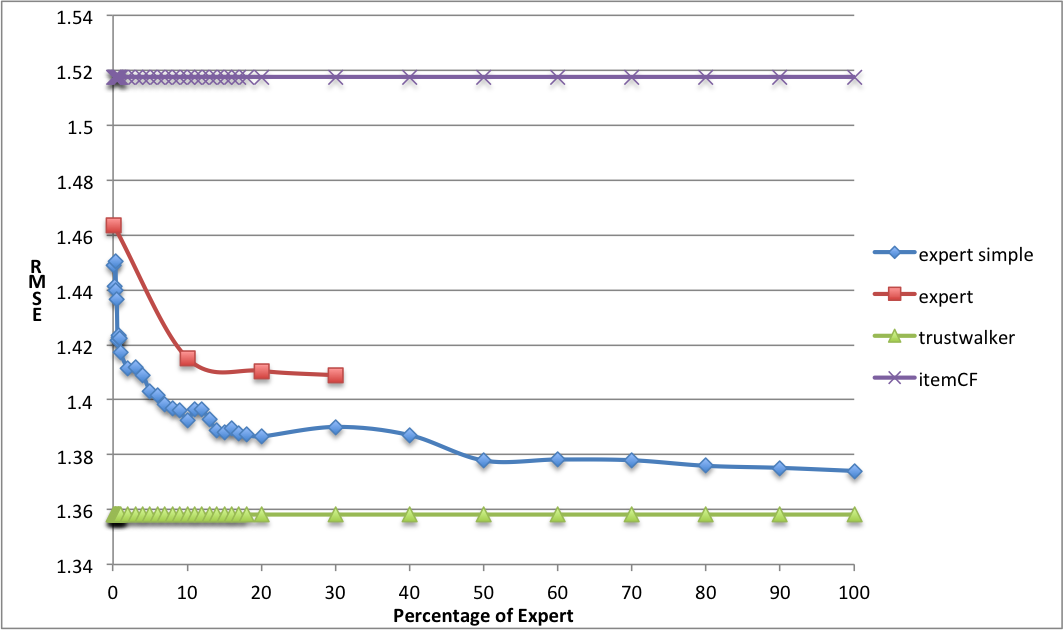
\includegraphics[width=12cm]{graphics/coldstart_user_2.png}			
	}
	\caption{RMSE Variation for Different Expert Percentage on ALL items}
	\label{fig:rmse_all}
\end{figure}

As shown in Figure \ref{fig:sub_rmse_all}, \emph{expert-simple} and \emph{expert} outperforms \emph{itemCF} and \emph{trustwalker} for all users with expert percentage larger than 1\%. And \emph{expert} gives a better start-off than \emph{expert-simple} but both of them seem to converge to the same RMSE as expert percentage becomes large. This is explainable because \emph{expert} not only considers the target item but also similar items. So with few experts, \emph{expert} could sample significantly more than \emph{expert-simple}. But with many experts, the difference of samples become smaller. As the expert percentage increases, the RMSE of both expert recommendation methods decrease. This is different from previous research \cite{Sarwar:2001p433} since we expected that the more experts we choose, the more the noise there would be and thus the RMSE should increase when expert percentage is larger than certain number. We believe that this rare behavior is caused by Epinions dataset. In our Epinions dataset ratings of 4 and 5 account for more than 60\% of the total ratings, and the average rating of our dataset is 3.95. Previous research has shown that employing simple method like always recommending 5 could achieve comparable performance to other sophisticated methods \cite{Massa:2007p437}. Thus not enough variety of ratings in our dataset gives shortcut for both expert recommenders to achieve good performance. But note that the expert methods are not personalized at all. In other words, for each user they would recommend exactly the same items while itemCF and TrustWalker are personalized methods.


Figure \ref{fig:sub_rmse_cold} shows the RMSE of the four methods over cold-start users. For cold-start users, item CF performs poorly, since it could not find enough rated similar items from the target user's rating profile. TrustWalker performs better than both expert methods. This result is expected, since TrustWalker was designed to mitigate the cold-start user's problem.


The other most widely used metric to evaluate recommender is coverage. Figure \ref{fig:results_all} shows the precision, coverage and F measure of all four methods over all users and cold-start users. The data of \emph{expert} method is for 30\% experts. The data of \emph{expert-simple} method is for 100\% experts.

In Figure \ref{fig:sub_results_all}, F-Measure of both expert methods are higher than TrustWalker and item-based CF, meaning that their overall performance is better than the latter two methods. The precision and coverage of \emph{expert} method is worse than those of \emph{expert-simple} method because the data of \emph{expert} method is measured with 30\% expert percentage while that of \emph{expert-simple} is measured at 100\%. As indicated by the trend in \ref{fig:sub_rmse_all}, the RMSE of \emph{expert} would probably converge with that of \emph{expert-simple}. The coverage of both expert methods are significantly better than item-based CF and 15\% better than TrustWalker. This is because the number of experts per category is significantly larger than a user's friends.

Figure \ref{fig:sub_results_cold} shows the performance of the four methods on cold-start users. The coverage of item-based CF is very low (only 15\%). TrustWalker greatly improves the coverage compared to item-based CF. Both expert methods are much better in terms of coverage because they do not differentiate between normal user and cold-start users. Thus the coverage for both types of users are almost the same. Notice that the precision of TrustWalker is the highest, though its F-Measure is not as high due to its smaller coverage. If we compare F-Measure, both expert methods are still the two highest.


\begin{figure}[htbp]
	\centering
	\subfloat[Results for ALL users on ALL items]{\label{fig:sub_results_all}
			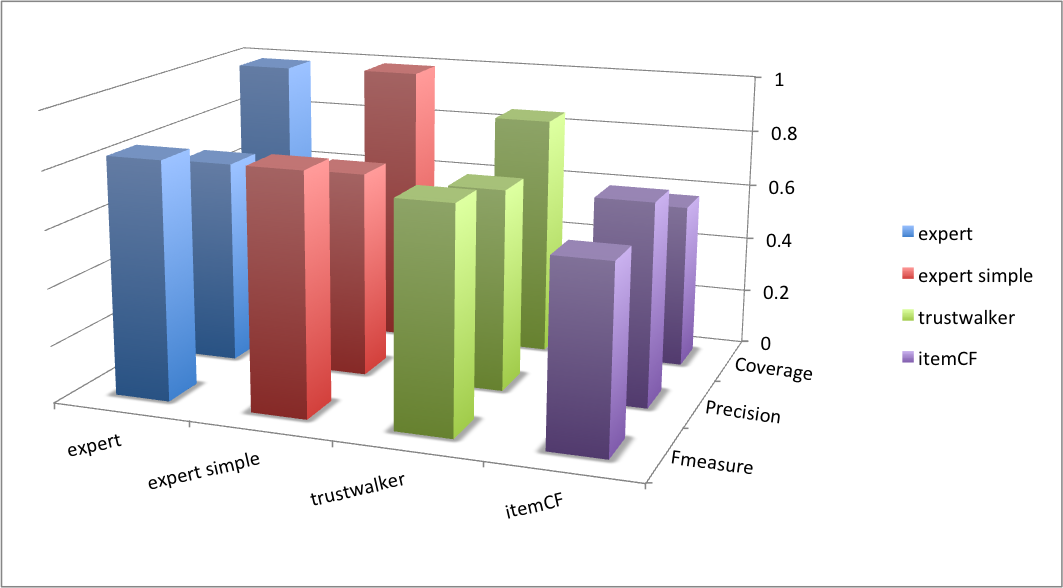
\includegraphics[width=12cm]{graphics/all_user.png}			
	}
	\\
	\subfloat[Results for COLD-START users on ALL items]{\label{fig:sub_results_cold}
			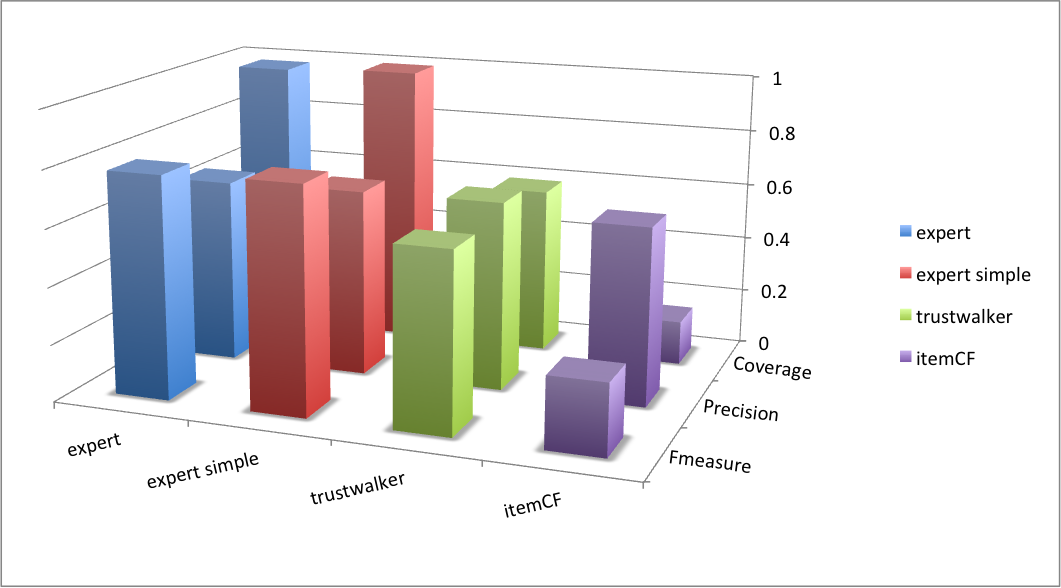
\includegraphics[width=12cm]{graphics/coldstart_user.png}			
	}
	\caption{Coverage, Precision and F-Measure for ALL Items}
	\label{fig:results_all}
\end{figure}

\begin{table}[htbp]
	\centering
	\subfloat[Experimental results for ALL users and ALL items \label{tbl:compare_all_all}]{
		\begin{tabular} {| c | c | c | c |  }
			\hline
			Method & RMSE & Coverage(\%) & F-Measure \\ \hline \hline
			expert & 1.222 & 98.79 & 0.832 \\ \hline
			expert-simple  & 1.112 & 99.56 & 0.837 \\ \hline
			itemCF & 1.170 & 57.84 & 0.636 \\ \hline
			trustwalker & 1.171 & 85.22 & 0.773 \\ \hline
			\hline
		\end{tabular}
	}
	\\
	\subfloat[Experimental results for COLD-START users and ALL items \label{tbl:compare_cold_all}]{
		\begin{tabular} {| c | c | c | c |  }
			\hline
			Method & RMSE & Coverage(\%) & F-Measure \\ \hline \hline
			expert & 1.409 & 97.93 & 0.780 \\ \hline
			expert-simple & 1.374 & 99.39 & 0.791 \\ \hline
			itemCF & 1.518 & 15.50 & 0.248 \\ \hline
			trustwalker & 1.358 & 58.97 & 0.623 \\ \hline
			\hline
		\end{tabular}
	}
	\caption{Experimental results for ALL items}
	\label{tbl:compare_all}
\end{table}

Since the performance of non-personalized expert methods are surprisingly good up to now, we tested all four methods on a subset of our testing set, which only contains \emph{controversial items}. We have already defined controversial items in previous section to be the items whose ratings' Standard Deviations are greater than 1.5. We expect \emph{expert} and \emph{expert-simple} to perform worse in this dataset since they are non-personalized methods and virtually give the average rating as prediction. Figure \ref{fig:con_all_user} shows the RMSE of the estimated ratings for controversial items. The performance of two personalized methods \emph{itemCF} and \emph{Trustwalker} are similar to the two non-personalized methods \emph{expert} and \emph{expert-simple}. Notice that in Table \ref{tbl:compare_controversial} the performance of \emph{expert} and \emph{expert-simple} has already decreased in terms of F-Measure compared to that in Table \ref{tbl:compare_all_all}. However, the performance of two personalized methods \emph{itemCF} and \emph{Trustwalker} also have performance degradation as expert methods. This means that even for controversial items where personalized methods are expected to perform much better, \emph{expert} and \emph{expert-simple} can still achieve comparable RMSE and higher coverage. 

\begin{table}[htbp]
	\centering
	%\subfloat[Experimental results for ALL users and CONTROVERSIAL items \label{tbl:compare_all_controversial}]{
		\begin{tabular} {| c | c | c | c |  }
			\hline
			Method & RMSE & Coverage(\%) & F-Measure \\ \hline \hline
			expert & 1.374 & 99.83 & 0.792 \\ \hline
			expert-simple & 1.406 & 99.25 & 0.785 \\ \hline
			itemCF & 1.414 & 47.33 & 0.546 \\ \hline
			trustwalker & 1.414 & 81.13 & 0.720 \\ \hline
			\hline
		\end{tabular}
	%}
	% \\
	% \subfloat[Experimental results for COLD-START users and CONTROVERSIAL items \label{tbl:compare_cold_controversial}]{
	% 	\begin{tabular} {| c | c | c | c |  }
	% 		\hline
	% 		Method & RMSE & Coverage(\%) & F-Measure \\ \hline \hline
	% 		expert & 1.686 & 99.83 & 0.733 \\ \hline
	% 		expert-simple & 1.666 & 98.61 & 0.733 \\ \hline
	% 		itemCF & 1.959 & 8.98 & 0.153 \\ \hline
	% 		trustwalker & 1.711 & 57.34 & 0.573 \\ \hline
	% 		\hline
	% 	\end{tabular}
	% }
	\caption{Experimental results ALL users on CONTROVERSIAL items}
	\label{tbl:compare_controversial}
\end{table}



\begin{figure}[htbp]
\centering
	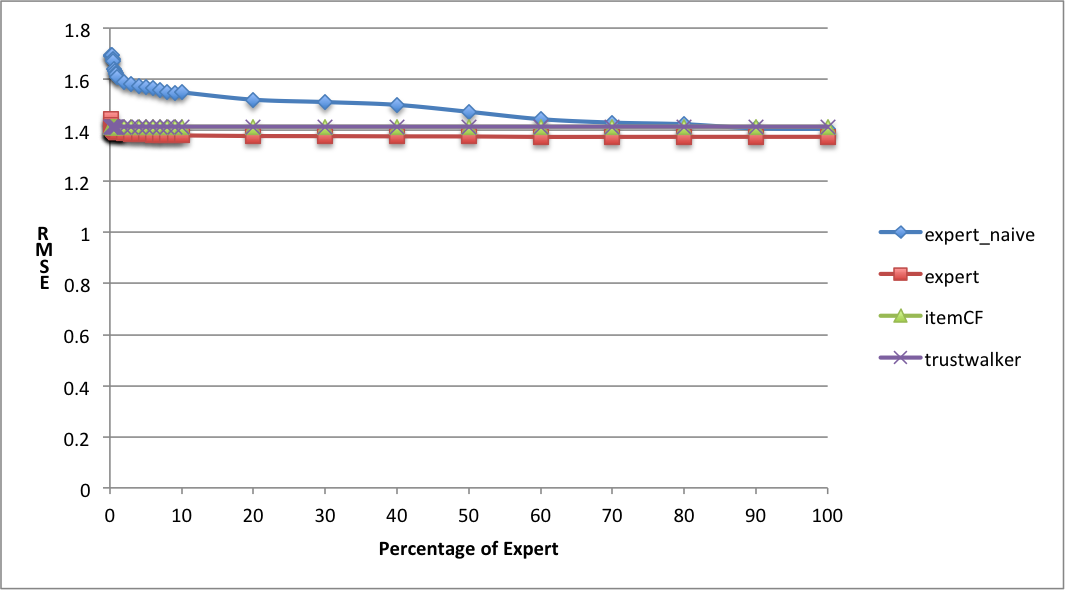
\includegraphics[width=12cm]{graphics/con_all_user.png}	
	\caption{RMSE of ALL uses on CONTROVERSIAL items}
	\label{fig:con_all_user}
\end{figure}


%%%%%%%%%%%%%%%%%%%%%%%%%%%%%%%%%%%%%%%%%%%%%%%%
% Section 4
%%%%%%%%%%%%%%%%%%%%%%%%%%%%%%%%%%%%%%%%%%%%%%%%
\section{Conclusion}
We calculate users' expertise using the number of qualities of their reviews. Then we pick users with highest expertise in each category and identify them as experts. We implemented two recommendation methods based on experts, and tested them against the dataset we crawled from Epinions.com. 

Initially we wanted to incorporate expertise of each user into TrustWalker and improve its accuracy. However, experiments show that this method is no better than original TrustWalker. On the other hand, more naive method \emph{expert} and \emph{expert-simple} perform surprisingly well in terms of both accuracy and coverage. This could be result of the nature of our dataset, in which ratings are clustered around 4 and 5. 

Based on our experiment results, we believe that more complicated method may not be necessary in some scenarios. For example, if the reviewed products are more objective and less subjective, simply averaging experts' opinions could be comparable or better to trust-based method. For subjective products like music and movies, more complicated and personalized method usually outperforms simple averaging and are desired. 

\bibliographystyle{ieeetr}
\bibliography{references}


\end{document}